\documentclass{article}

% pacakages
\usepackage{amsmath, amsfonts, amssymb}
\usepackage{stmaryrd}
\usepackage{fancyhdr}
\usepackage{lastpage}
\usepackage{lipsum}
\usepackage{graphicx}
\usepackage[ddmmyyyy]{datetime}
\usepackage[a4paper, portrait, margin=30mm]{geometry} % définie le format de la page

%code formatting
\usepackage{minted}
\usemintedstyle{manni}

%divers commands
\newcommand{\bb}[1]{\mathbb{#1}}
\newcommand{\encadrer}[1]{\fbox{
    \begin{minipage}{0.90\textwidth}
        #1
    \end{minipage}
}}
\renewcommand{\thesection}{\Roman{section}} %Roman numerals for sections

%page numerotation
\pagestyle{fancy}
\fancyhf{}
\renewcommand{\headrulewidth}{0pt}
\fancyfoot[R]{\thepage/\pageref{LastPage}} 

%document info
\makeatletter
\title{TD - Fil de priorité et Tas}
\date{\today}
\newcommand{\matiere}{Informatique}
\newcommand{\classe}{MP^*}
\author{Arsène MALLET}

%header
\fancypagestyle{firstpage}{
    \fancyhead[L]{\@author}
    \fancyhead[C]{\matiere}
    \fancyhead[R]{\@date}
}


\begin{document}

\thispagestyle{firstpage}

\begin{center}
    \huge{\@title}
\end{center}

\section{Un tas de question}

1.\begin{figure}[h]
    \centering
    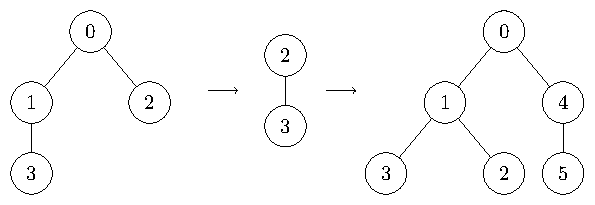
\includegraphics[scale=0.7]{drawing/I_1.pdf}
\end{figure}

2. 

3. \begin{minted}[breaklines]{ocaml}
    let rec is_tas_max heap = 
        test = ref true in
        for i = 0 to heap.n - 1 do
            if a.(i) > a.((i-1)/2) then
            test := false
        done;
        !test ;;
\end{minted}

4.

5. \begin{minted}{ocaml}
    let rec fusion l1, l2 = match l1, l2 with
        |[], _ -> l2
        |_, [] -> l1
        |e1::q1, e2::q2 -> if e1 < e2 then
                                e1::fusion q1 l2
                            else
                                e2::fusion l1 q2 
    ;;
\end{minted}

La complexité est $O(n+m)$
\begin{figure}[h]
    \centering
    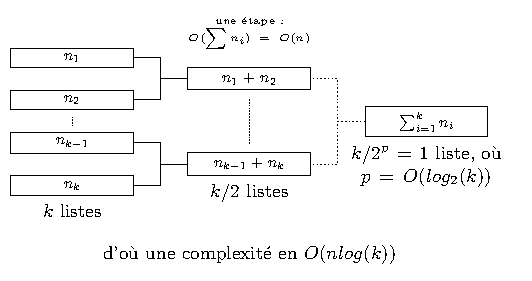
\includegraphics{drawing/I_5.pdf}
\end{figure}

\begin{minted}{ocaml}
    let rec etape ll = match ll with
        |l1::l2::q -> (fusion l1 l2)::etape q
        |_ -> ll 
    ;;

    let rec kfusion ll = match ll with
        |[] -> []
        |[l] -> l
        |_ -> kfusion (etape ll)
    ;;
\end{minted}

\section{Compression de Huffman}

\section{Arbretas}

1. \begin{minted}[]{ocaml}
    let swap t i j =
        let tmp = t.(j) in
        t.(j) <- t.(i); t.(i) <- tmp
    ;;
\end{minted}

2. La fonction \texttt{shuflle t} permutte tous les éléments du tableau \texttt{t} avec un autre éléments du tableau
choisi au hasard dans les indices inférieurs. Après avoir terminé la boucle \texttt{for}, le tableau a donc subit une permutation
aléatoires.

3. \begin{figure}[h]
    \centering
    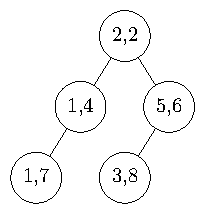
\includegraphics[scale = 0.7]{drawing/III_3.pdf}
    \end{figure}

4.

5. \begin{minted}{ocaml}
    let rotd treap = match treap with
    |N(r, N(gr, gg, gd), d) -> N(gr, N(r, gd, d), gg)
    |_ -> treap
\end{minted}

6. \begin{figure}[h]
    \centering
    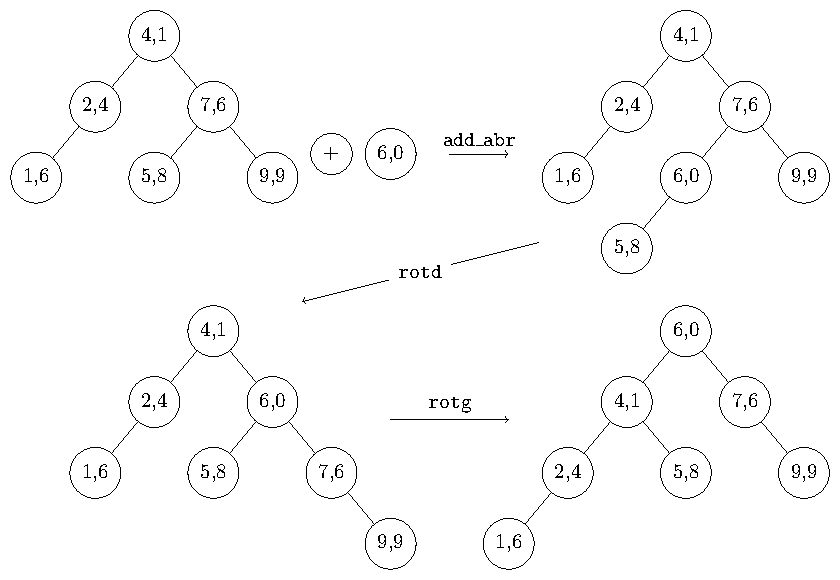
\includegraphics[scale=0.84]{drawing/III_6.pdf}
\end{figure}

7. \begin{minted}{ocaml}
    let prio tree = match tree with
    |V -> max_int
    |N((_, p), _, _) -> p
    ;;
\end{minted}

8. \begin{minted}{ocaml}
    let rec add treap e = 
      let elem, _ = e in
      match treap with
      |V -> N(e, V, V)
      |N((x, p), g, d) -> if elem >= x then 
                              let d_upt = add d e in
                                  if (prio d_upt) < p then
                                    rotg (N((x,p), g, d_upt))
                                  else N((x,p), g, d_upt)
                          else 
                              let g_upt = add g e in
                              if (prio g_upt) < p then
                                  rotd (N((x,p), g_upt, d))
                                else N((x,p), g_upt, d)
                                ;;
\end{minted}

9. \begin{minted}{ocaml}
    let rec del treap e = match treap with
    |V -> V
    |N((x,p), g, d) -> if e > x then
                        N((x,p), g, (del d e))
                      else if e < x then
                        N((x,p), (del g e), d)
                      else match g,d with
                        |V, V -> V
                        |V, f |f, V -> f
                        |_ -> if prio g < prio d then
                              let treap_rot = rotd(treap) in
                                del treap_rot e
                              else let treap_rot = rotg(treap) in
                                del treap_rot e
                            ;;
\end{minted}
\end{document}